\section{گرافیک کامپیوتری}

گرافیک کامپیوتری زیرشاخه‌ای از علوم کامپیوتر است که روش‌های 
ترکیب دیجیتالی و دستکاری محتوای بصری 
را مطالعه می‌کند.
اغلب اوقات این اصطلاح به مطالعه‌ی گرافیک 
کامپیوتری سه‌بعدی اشاره دارد \cite{ComputerGraphicsWikipedia}.
گرافیک کامیپوتری را می‌توان در 
موارد مختلفی مانند طراحی رابط کاربری،
رندر اشیاء هندسی، پویانمایی و بسیاری 
موارد دیگر استفاده کرد.
ابزارهای مختلفی برای پیاده‌سازی گرافیک کامپیوتری استفاده می‌شوند.
یکی از این ابزار‌ها 
\lr{OpenGL}
است.
در این پروژه برای ایجاد محیط گرافیکی از 
\lr{OpenGL}
استفاده شده است.
برای اینکه بتوان شخصیت‌ها و محیط سه‌بعدی را به وضوح مشاهده کرد از یک الگوریتم نورپردازی به نام 
سایه‌زنی فانگ استفاده شده است.
در این بخش توضیح کوتاهی دربا‌ره‌ی
 \lr{OpenGL}
 و
این روش سایه‌زنی آورده شده است.

\subsection {
    \lr{OpenGL}
    }

\lr{OpenGL}
یک واسط برنامه نویسی کاربردی  
\LTRfootnote{API}
است که با فراهم کردن توابع مختلف به توسعه‌دهندگان امکان دستکاری گرافیک و تصاویر را می‌دهد.
\lr{OpenGL} 
یک کتابخانه‌ی رندرینگ است.
یک "شئ" به خودی خود در
\lr{OpenGL} 
مفهومی ندارد
و به صورت مجموعه‌ای از مثلث‌ها و حالات مختلف درنظر گرفته می‌شود. بنابراین  
وظیفه‌ی ما است که بدانیم چه شئ‌ای در کدام قسمت صفحه رندر شده است. این کتابخانه تنها وظیفه‌اش، کشیدن تصاویری که است که می‌خواهیم به تصویر کشیده‌شوند.
در این صورت اگر می‌خواهیم تصویری را به‌روزرسانی کنیم و یا به عنوان مثال شئ‌ای را متحرک کنیم باید به 
\lr{OpenGL}
درخواست دهیم که صحنه را دوباره‌ برای ما رندر کند \cite{KhronosUsingOpenGL}.
به صورت کلی 
\lr{OpenGL}
را می‌توان یک ماشین حالت بزرگ درنظر گرفت. هر حالت شامل مجموعه‌ای از متغیر‌ها است که نحوه‌ی عملکرد
\lr{OpenGL}
را مشخص می‌کند. 
به مجموعه‌ی این حالت‌ها 
\lr{OpenGL context}
نیز می‌گویند. 
در واقع  
\lr{context}
را می‌توان یک شئ درنظر گرفت که کل
\lr{OpenGL}
را دربر می‌گیرد. عموما تمامی تغییرات، روی 
\lr{context}
فعلی اعمال می‌شود و سپس رندر می‌شود \cite{KhronosUsingOpenGL} \cite{LearnOpenGL_GettingStarted}.


\subsection{سایه‌زنی فانگ}
\label{PhongShading}
نورپردازی در دنیای واقعی بسیار پیچیده است و
به عوامل بسیار زیادی بستگی دارد. با توجه به 
قدرت محدود پردازش، برای ما چنین امکانی وجود ندارد که رفتار آن را 
به صورت کامل تخمین بزنیم.
بنابراین برای نورپردازی محیط‌های سه‌بعدی از تقریب‌ واقعیت 
با استفاده از مدل‌های ساده‌شده‌ی فیزیکی استفاده می‌شود.
یکی از این روش‌ها مدل سایه‌زنی فانگ نام دارد.
این مدل بر اساس سه مولفه‌ی اصلی عمل می‌کند.
این سه ‌مولفه، نورمحیطی
\LTRfootnote{Ambient light}
، نور پخش‌شده
\LTRfootnote{Diffuse light}
و نور آینه‌وار
\LTRfootnote{Specular light}
نام دارند \cite{LearnOpenGLPhongShading}.

\subsubsection{نورمحیطی}

نور معمولا از یک منبع نور منفرد ساطع نمی‌شود، بلکه
از منابع نوری زیادی که در اطراف ما پراکنده‌شده‌اند،
حتی زمانی که به صورت مستقیم قابل مشاهده‌نیستند،
نشات می‌گیرد.
حتی زمانی که هوا تاریک است، معمولا هنوز مقداری 
نور در جایی در جهان وجود دارد.
مانند ماه در هنگام شب.
بنابراین اجسام تقریبا هرگز به صورت کامل 
تاریک نیستند.
اگر بخواهیم چنین مولفه‌ای را به صورت واقعی مدل‌سازی کنیم، 
الگورتیمی بسیار پر هزینه خواهد بود.
به همین جهت در مدل فانگ برای اینکه بتوانیم نور محیطی را 
در اجسام سه بعدی مشاهده کنیم، 
از یک رنگ ثابت کوچک نور استفاده می‌کنیم و آن را به 
رنگ نهایی هر شئ اضافه می‌کنیم.
در این صورت به‌نظر می‌رسد که همیشه مقداری نور پراکنده در محیط 
سه‌بعدی وجود دارد \cite{LearnOpenGLPhongShading}.

\subsubsection{نور پخش‌شده}

می‌دانیم هرچه جسم به یک منبع نور نزدیک تر باشد و هرچه 
بخشی از یک جسم بیشتر به سمت منبع نور باشد، بیشتر روشن می‌شود.
این مولفه، تاثیر جهت قرار گیری 
اجسام نسبت به منبع نور را شبیه‌سازی می‌کند \cite{LearnOpenGLPhongShading}.

\subsubsection{نور آینه‌وار}

این مولفه وظیفه‌ی شبیه‌سازی نقطه‌ی روشن نوری که 
بر روی اجسام براق ظاهر می‌شوند، را دارد.
جهت قرار گیری اجسام نسبت به جهت نور 
تاثیر زیادی بر نحوه‌ی شکل گیری و شمایل این 
نقطه‌ی روشن‌شده دارد.
همچنین نحوه‌ی عملکرد نورپردازی آینه‌وار رابطه‌ی مستقیمی با 
 جنس سطح و خواص بازتابی آن سطح دارد.
هرچه سطح اجسام به جنس آینه‌ای نزدیک شود، نور بیشتری را بازتاب می دهد 
و بلعکس ممکن است جنس آن مانند گچی باشد که نور زیادی را جذب خود می‌کند \cite{LearnOpenGLPhongShading}.

در تصویر 
\ref{fig:PhongShadingWikipedia}
می‌توانیم عملکرد تمامی این مولفه‌ها را در مدل فانگ مشاهده کنیم.

\begin{figure}[ht]
	\centerline{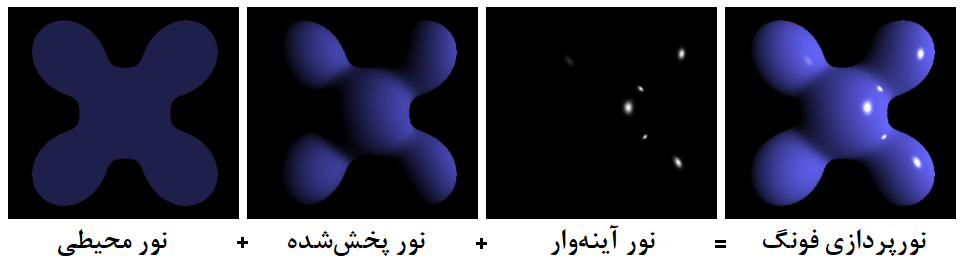
\includegraphics[width=\textwidth,height=\textheight,keepaspectratio]{Figures/Ch2/Phong_components.png}}

	\caption{مولفه‌های الگوریتم سایه‌زنی فانگ
    \cite{PhongShadingWikipedia}
    }
	\label{fig:PhongShadingWikipedia}
\end{figure}
